%For the uncoordinated multiple access problem we consider the non-asymptotic regime of fixed and finite number of users. Soliton distribution  is known to be optimal asymptotically but provides only a throughout of $\approx 0.75$ for $n=1000$. As far as we are aware the best known throughput in the literature is $0.82$. Although multiple random access schemes were proposed and studied the throughput performance is evaluated by numerical simulations. To the best of our knowledge there do not exist an analytic evaluation of performance of any random access scheme based on the content resolution decoding scheme. In this chapter we derive an analytical approximations for the probability of error . 

% and based on this approximation we devise a multiple round LP optimization scheme to find the optimal left degree distribution (based on which the users choose the number of time slots to transmit in). As of now with the aid of this scheme we are able to achieve a net throughput of $0.86$ for $n=1000$ which we also provide evidence for via Monte Carlo simulations.

\section{Motivation}
Recently, there has been a lot of interest in the design of random access strategies for the uncoordinated massive multiple access problem in view of wireless networks. An interesting connection has been established between codes on graphs and the decoding of multiple users (or, collision resolution in multiple access schemes). Leveraging this connection, many results from coding theory have been used to design and analyze various random access strategies. Particularly, it has been shown that in the limit of the number of users becoming asymptotically large, the throughput efficiency of uncoordinated multiple access can be as high as that of coordinated multiple access \cite{narayanan2012iterative}. In this chapter, we consider the non-asymptotic regime when the number of users is fixed and finite. By extending the finite-length analysis of low density parity check (LDPC) code ensembles \cite{amraoui2007find} to the multiple access case, we analyze the performance of the random access schemes for finite lengths and verify with numerical simulations.

\subsection{System model}
In the considered system model there are a total of $n$ users currently active each with one packet of information to transmit to the access point. Similar to Ch.~\ref{chap:MAC} the transmission period is partitioned into sub-blocks, referred to as slots, thus resulting in a similar slotted structure. Let the total number of slots available per round be $m$. The random access strategy of each user, independent and uncoordinated from other users, can be described as following. Each user $k$, $k\in [1:n]$, populates a random variable $D_{k}$ distributed according to the probability mass function $L(x)$ or equivalently $\Pr(D_{k}=i)=L_{i}$. The respective user then chooses $D_{k}$ time slots uniformly at random, with replacement, from the $m$ available slots. We will refer to this paradigm of picking check nodes randomly as \textit{uniform-with replacement} paradigm. We can represent the random strategy via bipartite Tanner graphs similar to a LDPC code where the variable nodes represent the $n$ users and the check nodes represent the $m$ available slots. There exists an edge between variable node $i$ and check node $j$ if and only if user $i$ chose to transmit in slot $j$. Note that we follow the same convention as used in describing LDPC codes for the degree distribution polynomials:
\begin{align}
L(x)=\sum_{i=1}^{l_{\text{max}}} L_{i}x^{i}\label{eqn:varnodedd_LDPC}\\
\lmb(x)=\sum_{i=1}^{l_{\text{max}}} \lmb_{i}x^{i-1},\notag
\end{align}
where $L(x)$ and $\lmb(x)$ denote variable node degree distributions, from node and edge perspectives respectively.
$R(x)$ and $\rho(x)$ are defined similarly for the check nodes. 
\begin{table}[!ht]
\centering
\begin{tabular}{|c|l|}
\hline
Notation & Parameter represented\\
\hline
$n$ & Total number of users in the system (variable nodes)\\ %which hereafter will also be referred to as variable nodes interchangeably.
$m$ & Number of time slots per one round of communication (check nodes)\\ % which hereafter also referred to as check nodes.
$L(x)$ & Variable node degree distribution, node perspective\\
$R(x)$& Check node degree distribution, node perspective\\
$\lambda(x)$ & Variable node degree distribution, edge perspective\\
$\rho(x)$& Check node degree distribution, edge perspective\\
$P_B$ & Prb. that $n$ users are not decoded successfully \\
$P_b$ & Prb. that a random user is not decoded successfully \\
\hline
\end{tabular}
\caption{Summary of parameters encountered in this chapter along with the notation used is given above.}
\label{table:notaiton_randomMAC}
\end{table}
For a given $n, L(x)$ probability that a randomly generated graph is not decoded completely by successive interference cancellation decoder (see peeling decoder \cite{richardson2008modern}) referred to as probability of block error $P_{B}$. Similarly the probability that a random user in a session is failed to be decoded by the access point as probability of bit error $P_{b}$.

 
\section{Review}
We start with a review of the existing results in the analysis of error performance of finite-length LDPC codes over binary erasure channel (BEC) under peeling decoder. Most of these results are due to Amraoui, Montanari and Urbanke \cite{amraoui2007find}.

Consider an LDPC  $(n,\lmb,\rho)$ ensemble which can be defined as the ensemble of bipartite graphs with $n$ variable nodes, $m$ check nodes, and edge connections are formed randomly such that the variable and check node d.d's are $\lambda(x)$, $\rho(x)$ respectively. For more details refer \cite{richardson2008modern}. Luby et al, \cite{luby1997practical} analyzed the peeling decoder and computed expressions for the evolution of expected number of degree-one check nodes as a function of the size of the residual graph, as the peeling algorithm progresses. More precisely, let $\tilde{R}_{1}(y)$ denote the fraction of degree-one check nodes (as a fraction of $m$- number of check nodes in the original graph) present in the residual graph. Here the number of degree-one check nodes in the residual graph is given in parametric form where $y$ is a function of the number of edges peeled off. Note that $t=0$ corresponds to $y=1$ and $t\rightarrow \infty$ corresponds to $y\rightarrow 0$. Then
\begin{align}
\tilde{R}_{1}(y)=R'(1)\epsilon\lmb(y)[y-1+\rho\left(1-\epsilon\lmb(y)\right) ].
\label{Eqn:Residual}
\end{align}
For a $(3,6)$ regular LDPC code, the average number of degree-one check nodes given by \eqref{Eqn:Residual} is plotted in Fig. \ref{Fig:LDPCResidual}. Note that the figure is reproduced from \cite{amraoui2007find}.

\begin{figure}[!ht]
\centering
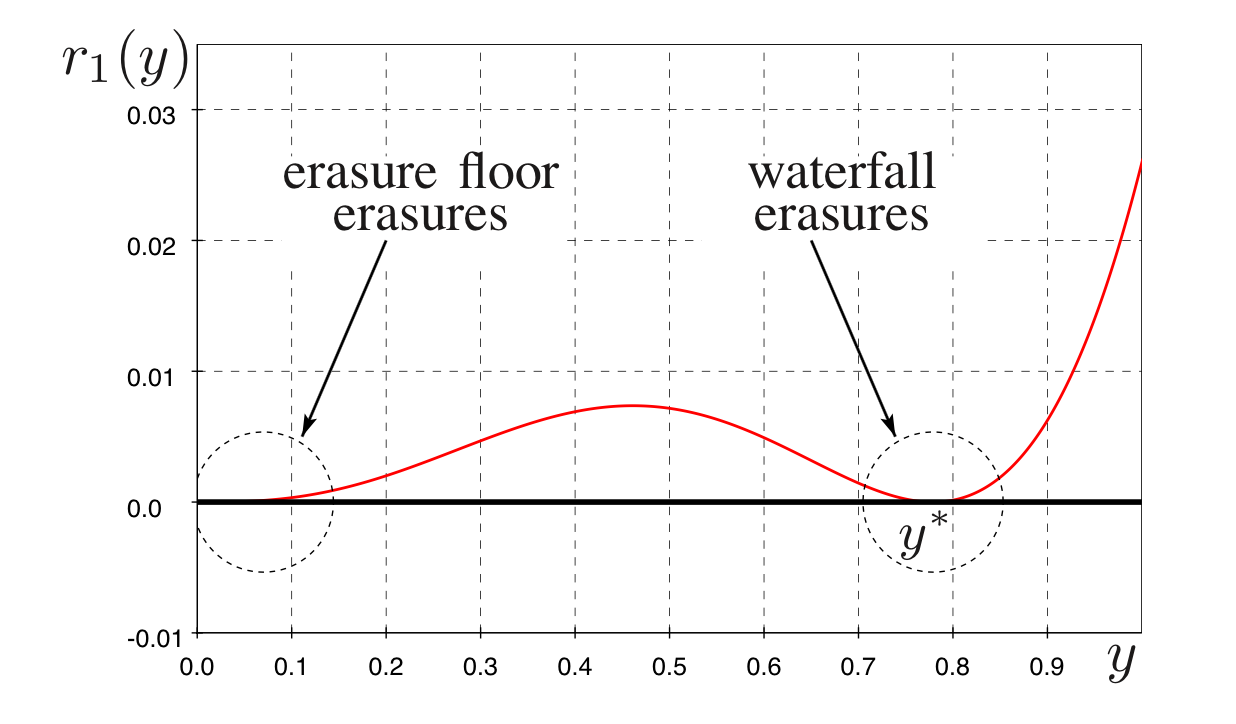
\includegraphics[width=0.85\textwidth]{data/UMAC/Figures/small_large_Erasures.png}
\caption{$\tilde{R}_{1}(y)$ at $\epsilon=\epsilon_{\text{BP}}$ for $\lmb(x)=x^2,\rho(x)=x^5$. Note that this figure is reproduced from \cite{amraoui2007find}.}
\label{Fig:LDPCResidual}
\end{figure}

%\subsection{Error probability approximates}
 The authors \cite{amraoui2007find} demonstrate that (can also be observed from Fig. \ref{Fig:LDPCResidual}) the failure of decoder occurs with high probability in two possible scenarios: The first case corresponds to $y\approx 0$ or as $t\rightarrow \infty$ and the other case corresponds to the value of $y$ such that $\tilde{R}_{1}(y)=0$ when $\epsilon=\epsilon_{\text{BP}}$ or equivalently at the value of $y$ where the curve has a stationary point. This point is referred to as critical point $y^*.$ The errors caused corresponding to the first case are referred to as \textit{small-error} events or error floor erasures since they occur towards the end of peeling decoder and the errors corresponding to the second case are referred to as \textit{large-error} events or waterfall erasures. The authors approximate the total probability of error by two expressions, each one corresponding to the one of these two cases.
 
%\subsubsection*{LP to increase the net throughput}~\\ \\ $\max \frac{-(1-P_b)}{m^2}\Delta m+\sum_{i}-\frac{\partial P_b•}{m\partial L_i}\Delta L_i- \frac{~\partial P_b}{m\partial m}\Delta m$
%\begin{align*}
%&\sum \Delta L_i=0;      & -\min\{\delta,L_{i}\}\leq \Delta L_i\leq \delta
%\end{align*}

\begin{theorem}[Scaling Law \cite{richardson2008modern}]
Consider transmission over a BEC channel using random elements from the LDPC $(n,\lambda,\rho)$ ensemble. Assume that the ensemble has a single critical point $y^*>0$ and let $\nu^*=\epsilon_{\text{BP}}L(y^*)$. Let $P_{\text{B}}^{W}(n,\lmb,\rho,\epsilon)$ denote the expected block erasure probability due to erasures of size atleast $n\gamma \nu^{*}$, where $\gamma\in (0,1)$. Fix $z:=\sqrt{n}(\epsilon_{\text{BP}}-\beta n^{-2/3}-\epsilon)$. Then as $n\rightarrow \infty ,$
\begin{align*}
P_{\text{B}}^{W}(n,\lmb,\rho,\epsilon)=Q\left(\frac{z}{\alpha}\right)\left(1+O(n^{-1/3})\right)
\end{align*}
where $\alpha$ and $\beta$ are constants dependent on the degree distributions.
\end{theorem}
The expression above approximates the error probability of large-erasure events.

\begin{theorem}[Error Floor \cite{amraoui2007find}]
Consider transmission over a BEC channel using random elements from the LDPC $(n,\lambda,\rho)$ ensemble. Assume that the ensemble has a single critical point $y^*>0$ and let $\nu^*=\epsilon_{\text{BP}}L(y^*)$. Let $P_{\text{B}}^{F}(n,\lmb,\rho,\epsilon)$ denote the expected block erasure probability due to stopping sets of size between $s_{\text{min}}$ and  $n\gamma \nu^{*}$, where $\gamma\in (0,1)$. Then for any $\epsilon<\epsilon_{\text{BP}}$
\begin{align*}
P_{\text{B}}^{F}(n,\lmb,\rho,\epsilon)=1-e^{-\sum_{s\geq s_{min}}\tilde{A}_{s}\epsilon^s}\left(1+o(1)\right),
\end{align*}
where $\tilde{A}_{s}=\text{coef}\{\log(A(x)),x^s\}$ for $s\geq 1$, with $A(x)=\sum_{s\geq 0} A_{s}x^s$ and
\begin{multline}
A_{s}=\sum_{e}\left( \text{coef}\left\lbrace\prod_{i} (1+xy^{i})^{nL_{i}}, x^{s}y^{e} \right\rbrace \right.\times \\
\left.\frac{\text{coef}\lbrace \prod_{i}\left((1+x)^i -ix \right)^{n(1-r)R_{i}},x^{e}\rbrace}{\binom{nL'(1)}{e}}\right).
\end{multline}
\end{theorem}
Note that $A_{s}$ is the expected number of stopping sets of size $s$ in a random graph picked uniformly at random from the graph and $\tilde{A}_{s}$ is the expected number of minimal stopping sets of size $s$. Following along similar lines we derive error floor expression in the case of random multiple access problem.
 
%Our objective is, for a given $n$, to minimize the total throughput $\eta=\frac{n}{m}\left(1-P_{b}(n,L(x)\right)$ over the variables $m$-number of slots and the degree distribution $L(x)$. Even from the analytical approximate expression for the bit/block probability of error it appears to be a highly complex problem and the global optimization would be very difficult to compute. So for a fixed $n$ and an initial left distribution $L(x)$ we compute the partial derivatives and implement the local optimization via LP to derive a locally optimal left distribution $L^{*}(x)$. With this as our current input to the LP we repeat the procedure until there are diminishing improvements to the total throughput $\eta$.

\section{Error analysis for random multiple access}
  We note that in the case of random uncoordinated multiple access scheme since the right degree distribution is not a design choice but rather has a Poisson distribution, as discussed in \cite{narayanan2012iterative}, the error probability approximations do not carry over directly from \cite{amraoui2007find} especially for the \textit{water-fall} erasures. But we approximate the small-error events $P_{\text{b}}^{\text{F}}(n,L)$, where `F' stands for error floor, the expression for which is given in \ref{sec:UMACapproximate}. We avoid the large error events by imposing a constraint in the optimization problem that the residual degree-1 check nodes $\tilde{R}_1(y)$ in the initial stages of peeling decoder is bounded away from $0$ by a certain threshold and thus the overall probability of error is well approximated by $P_{\text{b}}^{\text{F}}(n,L)$ alone. We support this claim by providing evidence via simulations.

%We consider the paradigm in which $k^{\text{th}}$ user/bit-node, for $k\in [1:n]$, generates a random variable $D_{k}$ from the probability mass function $L(x)$ independent of other bit nodes or equivalently $\text{Pr}(D_{k}=i)=L_{i}$. Each bit node, after the generation of $D_{k}$, chooses $D_{k}$ time slots/check nodes uniformly at random, with replacement, from the $m$ check nodes available. 

We will refer to the random access paradigm of picking check nodes randomly but with replacement as \textit{uniform-with replacement} paradigm. Even though the ``uniform-with replacement" allows for multiple edges in the graph, the analysis is made easier because of this assumption. For a given edge, probability that it connects to any of the check nodes is equal to $\frac{1}{m}$. We also believe that the resulting analysis can be easily extended to the ``uniform-without replacement" paradigm where in the $D_{k}$ check nodes are picked uniformly at random, but without replacement from the $m$ check nodes. Note that in Narayanan, Pfister \cite{narayanan2012iterative} consider the `` uniform-without replacement" paradigm. We define the ensemble of graphs for the random multiple access problem as UMAC$(n,\lmb,\eta)$ where $L(x)$ is as described in Eqn.~\eqref{eqn:varnodedd_LDPC}, is related to $\lmb(x)$ via
\begin{align*}
L(x)=\frac{\int_{0}^{x}\lmb(x)}{\int_{0}^{1}\lmb(x)}.
\end{align*}
 $\eta$ is the throughput ($n=m\eta$) and the edges are chosen as in the ``uniform-without replacement" paradigm.

\subsection{Error probability approximates}
\label{sec:UMACapproximate}
\begin{theorem}[Small error events]
Consider transmission by users over a noiseless MAC channel according to a graph picked uniformly at random from the UMAC$(n,\lmb,\eta)$ ensemble. Assume that the ensemble has no critical point i.e the degree-one check nodes in the residual graph is a monotonously decreasing function of time. Let $P_{\text{B},s_{min}}^{F}(n,\lmb,\rho,\epsilon)$ denote the expected block erasure probability due to stopping sets of size between $s_{min}$ and  $\gamma n$, where $\gamma\in (0,1)$. Then
\begin{align}
P_{\text{B},s_{min}}^{F}(n,\lmb,\rho,\epsilon)=1-e^{-\sum\limits_{s\geq s_{\text{min}}}^{\gamma n}\tilde{A}_{s}}\left(1+o(1)\right),
\label{Eqn:PBAnalytic}
\end{align}
where $\tilde{A}_{s}=\text{coef}\{\log(A(x)),x^s\}$ for $s\geq 1$, with $A(x)=\sum_{s\geq 0} A_{s}x^s$ and
\begin{multline}\label{Eqn:AvgSS}
A_{s}=\sum_{i}\left(\text{coef}\left\lbrace (1+x\sum_{i}L_{i}y^{i})^{n}, x^{s}y^{i} \right\rbrace \right.\times \\
\left.\frac{\text{coef}\lbrace (e^x -x)^{m},x^{i}\rbrace }{\frac{m^i}{i!}}\right). \\
\end{multline}
\label{Thm:UMACFloor}
\end{theorem}

\begin{proof}
We now give only a brief glimpse of the proof, the detailed proof will be added later. We first show that the expression for $A_{s}$ in \eqref{Eqn:AvgSS} is equal to the expected number of stopping sets of size `$s$' in a graph picked uniformly at random from the UMAC($n,\lmb,\eta$) ensemble. The first term is $\binom{n}{s}$ times the probability that $s$ nodes have $e$ edges attached to them and the second term is equal to the probability that the $e$ edges, under the ``uniform-with replacement" paradigm, form a stopping set i.e, they choose check nodes such that none of the check nodes chosen have only one edge connection.

From there we will try to follow the similar argument as in \cite{richardson2008modern} that for large values of $n$ the minimal stopping sets tend to a Poisson distribution with independent components. And then the relation between $A(x)$ and $\tilde{A}(x)$, expression for block/bit error probability follows along the same lines.
\end{proof}

\begin{remark}
Even though the condition in Theorem \ref{Thm:UMACFloor} that the degree-1 check nodes in the residual graph decrease monotonously with time is a stringent constraint to be satisfied, we believe that even when the curve of degree-1 check nodes has a stationary  point (curve $\tilde{R}_{1}(y)$ is non-monotonous function of $y$) the expression in Eqn. \eqref{Eqn:AvgSS}  approximates the probability of small error events well enough.
\end{remark}

\subsection{Results}
We use the following degree distribution, with a maximum degree of 30. Note that we chose this distribution randomly.
\begin{multline}
L_1(x)=0.3x^2+ 0.25 x^3+ 0.2 x^4 + 0.1 x^5+ 0.05 x^{10} + 0.04 x^{15}\\
 + 0.03 x^{20} + 0.02 x^{25}+ 0.01 x^{30}.
\label{Eqn:L1x}
\end{multline}
For the parameters of $n=1000, m=1300( \eta \approx 0.77)$ and $L(x)$ in Eqn. \eqref{Eqn:L1x} we get the following results given in Table.~\ref{Table:SimvsAnalytic1}. Note that $P_{B,s_{\text{min}}}^F$ is computed using the analytic expression given in \eqref{Eqn:PBAnalytic} whereas $P_{B,s_{\text{min}}}^{\text{Sim}}$ is computed using numeric simulations of Peeling decoder.


\begin{figure}
\centering
\setlength\figurewidth{0.8\columnwidth}
\setlength\figureheight{0.6\columnwidth}
% This file was created by matlab2tikz v0.4.7 running on MATLAB 7.14.
% Copyright (c) 2008--2014, Nico Schlömer <nico.schloemer@gmail.com>
% All rights reserved.
% Minimal pgfplots version: 1.3
% 
% The latest updates can be retrieved from
%   http://www.mathworks.com/matlabcentral/fileexchange/22022-matlab2tikz
% where you can also make suggestions and rate matlab2tikz.
% 
\begin{tikzpicture}

\begin{axis}[%
width=\figurewidth,
height=\figureheight,
scale only axis,
xmin=0,
xmax=1,
xlabel={Iterations},
xmajorgrids,
ymin=-40,
ymax=200,
ylabel={Residual Degree-1 Check Nodes},
ymajorgrids,
legend style={at={(0,1)},anchor=north west,draw=black,fill=white,legend cell align=left}
]
\addplot [color=red,solid,line width=1.5pt]
  table[row sep=crcr]{0	0\\
0.01	0.0324342999246084\\
0.02	0.130205815361465\\
0.03	0.293987817090611\\
0.04	0.524410156505397\\
0.05	0.822054268200592\\
0.06	1.18744801438634\\
0.07	1.62106039064647\\
0.08	2.12329611484881\\
0.09	2.69449012337941\\
0.1	3.33490200129503\\
0.11	4.0447103754538\\
0.12	4.8240073021706\\
0.13	5.67279268342755\\
0.14	6.59096874812536\\
0.15	7.57833463725704\\
0.16	8.63458113419017\\
0.17	9.7592855834234\\
0.18	10.951907043196\\
0.19	12.2117817191437\\
0.2	13.5381187277618\\
0.21	14.9299962397182\\
0.22	16.3863580540202\\
0.23	17.9060106546155\\
0.24	19.4876208011846\\
0.25	21.1297137055917\\
0.26	22.8306718446789\\
0.27	24.5887344587651\\
0.28	26.4019977833131\\
0.29	28.2684160587129\\
0.3	30.1858033599693\\
0.31	32.1518362842367\\
0.32	34.164057529585\\
0.33	36.219880393077\\
0.34	38.3165942101612\\
0.35	40.4513707504974\\
0.36	42.6212715776194\\
0.37	44.823256371239\\
0.38	47.0541922015086\\
0.39	49.3108637340943\\
0.4	51.5899843334615\\
0.41	53.8882080192293\\
0.42	56.202142216772\\
0.43	58.5283612282931\\
0.44	60.8634203342801\\
0.45	63.2038704173866\\
0.46	65.5462729812106\\
0.47	67.8872154148936\\
0.48	70.2233263306744\\
0.49	72.5512907751393\\
0.5	74.8678650854909\\
0.51	77.1698911291758\\
0.52	79.4543096280644\\
0.53	81.7181722262746\\
0.54	83.9586519127884\\
0.55	86.1730513551339\\
0.56	88.3588086372915\\
0.57	90.5134998221086\\
0.58	92.6348376740633\\
0.59	94.720665780088\\
0.6	96.7689471918946\\
0.61	98.7777465800384\\
0.62	100.745204734634\\
0.63	102.669504066718\\
0.64	104.548823553981\\
0.65	106.381281331209\\
0.66	108.164862845722\\
0.67	109.897332178663\\
0.68	111.576123773185\\
0.69	113.198211412465\\
0.7	114.759950861394\\
0.71	116.256892141816\\
0.72	117.683556981988\\
0.73	119.033176617602\\
0.74	120.297384908265\\
0.75	121.465861803666\\
0.76	122.525922757217\\
0.77	123.462051063987\\
0.78	124.255372784973\\
0.79	124.883078650327\\
0.8	125.317805215192\\
0.81	125.527000210276\\
0.82	125.472316889248\\
0.83	125.109112717954\\
0.84	124.386173978577\\
0.85	123.245856810552\\
0.86	121.624936521538\\
0.87	119.456603397797\\
0.88	116.674250532317\\
0.89	113.217985052458\\
0.9	109.045174254886\\
0.91	104.146817251678\\
0.92	98.5720866215064\\
0.93	92.4639285313235\\
0.94	86.108949459999\\
0.95	80.004586182306\\
0.96	74.9451636677844\\
0.97	72.125118791915\\
0.98	73.2517287294828\\
0.99	80.6513121779363\\
1	97.3445263373793\\
};
\addlegendentry{$L_1(x),\eta=0.77$};

\addplot [color=blue,solid,line width=1.5pt]
  table[row sep=crcr]{0	-0\\
0.01	0.0324342999454241\\
0.02	0.130205816540216\\
0.03	0.293987828713633\\
0.04	0.524410211361817\\
0.05	0.822054436379727\\
0.06	1.18744839020242\\
0.07	1.62106101023381\\
0.08	2.12329674311493\\
0.09	2.69448982841213\\
0.1	3.33489841199594\\
0.11	4.04469849414493\\
0.12	4.82397771825418\\
0.13	5.67272900696705\\
0.14	6.59084405359321\\
0.15	7.57810667783715\\
0.16	8.63418605615414\\
0.17	9.7586298384885\\
0.18	10.9508571647491\\
0.19	12.2101515961551\\
0.2	13.5356539785588\\
0.21	14.9263552570484\\
0.22	16.3810892635637\\
0.23	17.8985255019548\\
0.24	19.4771619579028\\
0.25	21.1153179644249\\
0.26	22.8111271573443\\
0.27	24.5625305591447\\
0.28	26.3672698340911\\
0.29	28.2228807624179\\
0.3	30.1266869868122\\
0.31	32.0757940903889\\
0.32	34.0670840719254\\
0.33	36.0972102913402\\
0.34	38.1625929663138\\
0.35	40.2594153096284\\
0.36	42.3836204062868\\
0.37	44.53090893983\\
0.38	46.6967378885548\\
0.39	48.8763203246001\\
0.4	51.0646264621615\\
0.41	53.256386115464\\
0.42	55.4460927425935\\
0.43	57.6280092678901\\
0.44	59.7961758933262\\
0.45	61.9444201281343\\
0.46	64.0663692858302\\
0.47	66.155465718642\\
0.48	68.2049850810613\\
0.49	70.2080579365958\\
0.5	72.1576950445935\\
0.51	74.0468166869157\\
0.52	75.8682864168572\\
0.53	77.6149496345894\\
0.54	79.2796774139531\\
0.55	80.8554160239703\\
0.56	82.3352426042164\\
0.57	83.7124274653064\\
0.58	84.9805034932132\\
0.59	86.1333431379365\\
0.6	87.1652434620313\\
0.61	88.0710197116236\\
0.62	88.8461078507147\\
0.63	89.4866764678907\\
0.64	89.9897484223778\\
0.65	90.3533325433943\\
0.66	90.5765656332882\\
0.67	90.6598649520345\\
0.68	90.6050912804597\\
0.69	90.4157225754979\\
0.7	90.0970381480775\\
0.71	89.6563132202427\\
0.72	89.1030236627827\\
0.73	88.4490606911378\\
0.74	87.7089553225666\\
0.75	86.9001124927707\\
0.76	86.0430549217833\\
0.77	85.1616771389922\\
0.78	84.2835105643373\\
0.79	83.4400012426543\\
0.8	82.6668027943376\\
0.81	82.0040884396886\\
0.82	81.4968876468592\\
0.83	81.1954551232481\\
0.84	81.1556826049878\\
0.85	81.4395672936855\\
0.86	82.1157549444023\\
0.87	83.2601806270451\\
0.88	84.9568361654408\\
0.89	87.2987002943643\\
0.9	90.3888757323577\\
0.91	94.3419866749835\\
0.92	99.285900631951\\
0.93	105.363849925412\\
0.94	112.73704025256\\
0.95	121.587846004979\\
0.96	132.123703765158\\
0.97	144.581825449799\\
0.98	159.234859404874\\
0.99	176.397629401307\\
1	196.435075586923\\
};
\addlegendentry{$L_2(x),\eta=0.77$};

\addplot [color=green,solid,line width=1.5pt]
  table[row sep=crcr]{0	0\\
0.01	0.0258363854806183\\
0.02	0.10328147936136\\
0.03	0.232180465548624\\
0.04	0.412295746914854\\
0.05	0.643301284286838\\
0.06	0.924776895131598\\
0.07	1.25620254462867\\
0.08	1.63695266473375\\
0.09	2.06629053978564\\
0.1	2.54336280015728\\
0.11	3.06719406837351\\
0.12	3.63668180497762\\
0.13	4.25059140418947\\
0.14	4.90755159201914\\
0.15	5.60605018193617\\
0.16	6.34443024540351\\
0.17	7.12088675651487\\
0.18	7.93346377157502\\
0.19	8.78005220569002\\
0.2	9.65838826922263\\
0.21	10.566052627285\\
0.22	11.5004703452196\\
0.23	12.4589116822184\\
0.24	13.4384937938054\\
0.25	14.4361834018069\\
0.26	15.448800487628\\
0.27	16.4730230610944\\
0.28	17.5053930527862\\
0.29	18.5423233726491\\
0.3	19.5801061716993\\
0.31	20.6149223368319\\
0.32	21.6428522410704\\
0.33	22.659887763072\\
0.34	23.6619455803104\\
0.35	24.6448817300991\\
0.36	25.6045074215048\\
0.37	26.5366060692219\\
0.38	27.4369515076605\\
0.39	28.3013273298053\\
0.4	29.1255472808813\\
0.41	29.9054766214382\\
0.42	30.6370543581812\\
0.43	31.316316223638\\
0.44	31.9394182675541\\
0.45	32.5026609036361\\
0.46	33.0025132348499\\
0.47	33.4356374587621\\
0.48	33.7989131312368\\
0.49	34.0894610419457\\
0.5	34.3046664283566\\
0.51	34.4422012257884\\
0.52	34.5000450194179\\
0.53	34.4765043292729\\
0.54	34.3702298207703\\
0.55	34.1802309905898\\
0.56	33.9058878299362\\
0.57	33.5469589137436\\
0.58	33.1035853042668\\
0.59	32.5762895899212\\
0.6	31.9659693043004\\
0.61	31.273883885283\\
0.62	30.5016342395385\\
0.63	29.6511338735247\\
0.64	28.7245704390083\\
0.65	27.7243564213245\\
0.66	26.6530675760932\\
0.67	25.5133676021811\\
0.68	24.3079174371861\\
0.69	23.0392674954878\\
0.7	21.7097311669398\\
0.71	20.3212380004924\\
0.72	18.8751652768365\\
0.73	17.3721472239657\\
0.74	15.8118620902465\\
0.75	14.1927988652998\\
0.76	12.5120079237899\\
0.77	10.7648436817441\\
0.78	8.94471309749036\\
0.79	7.04285236422604\\
0.8	5.04816661144334\\
0.81	2.94718549755974\\
0.82	0.72421347887326\\
0.83	-1.63820970755115\\
0.84	-4.15837126603556\\
0.85	-6.85373189389589\\
0.86	-9.73822137652723\\
0.87	-12.8180192202839\\
0.88	-16.0851907616107\\
0.89	-19.5083461089709\\
0.9	-23.0192582796967\\
0.91	-26.4941480676831\\
0.92	-29.7281825415224\\
0.93	-32.4017635113411\\
0.94	-34.0375972213806\\
0.95	-33.9486014601399\\
0.96	-31.1786855215329\\
0.97	-24.4413895725551\\
0.98	-12.0647201528052\\
0.99	8.04756732743722\\
1	38.4311186492295\\
};
\addlegendentry{$L_1(x),\eta=0.95$};

\end{axis}
\end{tikzpicture}%
\caption{$\tilde{R}_{1}(y)$ for UMAC($1000,L(x),0.77$) corresponding to $L_{1,2}(x)$ in Eqn. \eqref{Eqn:L1x}.}
\label{Fig:UMAC_Residual}
\end{figure}

\begin{table}
\centering
\begin{tabular}{c c c c c}
\hline  \hline
smin & $P_{B,\text{smin}}^F$ & $P_{B,\text{smin}}^{\text{Sim}}$ & $P_{b,\text{smin}}^F$ & $P_{b,\text{smin}}^{\text{Sim}}$ \\
\hline
2 & 7.89$\times 10^{-2}$  &  7.97$\times 10^{-2}$ &$2.13\times 10^{-4}$&$2.12\times 10^{-4}$\\
3 & 2.78$\times 10^{-2}$  & 2.84$\times 10^{-2}$&$1.05\times 10^{-4}$&$1.09\times 10^{-4}$ \\
4 & 1.11$\times 10^{-2}$  &1.30$\times 10^{-2}$ &$5.41\times 10^{-5}$&$6.33\times 10^{-5}$\\
5 & 4.80$\times 10^{-3}$  &5.90$\times 10^{-3}$& $2.88\times 10^{-5}$&$3.49\times 10^{-5}$\\
6 & 2.23$\times 10^{-3}$  &3.00$\times 10^{-3}$ &$1.58\times 10^{-5}$&$2.04\times 10^{-5}$\\
7 & 1.10$\times 10^{-3}$  &1.50$\times 10^{-3}$ &$9.04\times 10^{-6}$&$1.14\times 10^{-5}$\\
8 &5.68$\times 10^{-4}$   &5.00$\times 10^{-3}$&$5.28\times 10^{-6}$&$4.40\times 10^{-6}$\\
9 & 3.03$\times 10^{-4}$  &3.00$\times 10^{-4}$ & $3.15\times 10^{-6}$&$2.80\times 10^{-6}$\\
10 & 1.66$\times 10^{-4}$ &1.00$\times 10^{-4}$&$1.90\times 10^{-6}$&$1.00\times 10^{-6}$\\
\end{tabular}
\caption{Comparison of Probability of Block\textbackslash Bit errors computed analytically and via simulations for $L_1(x)$ given by Eqn. \eqref{Eqn:L1x}, $K=1000, \eta=0.77$.}
\label{Table:SimvsAnalytic1}
\end{table}

We notice that the analytic and numerical results are almost in perfect agreement. To justify applying Thm. \ref{Thm:UMACFloor} we verify that most of the error events are of small size, analytically through Fig.~\ref{Fig:UMAC_Residual}. We also verify numerically that the maximum stopping set size we observe is 22 thus rendering an approximation for error probability because of large error events unnecessary. \\

To verify for another distribution, we perform the experiments for another bit-node distribution given in Eqn. \eqref{Eqn:L2x}. The evolution of residual degree-1 check nodes is given in Fig. \ref{Fig:UMAC_Residual}. The corresponding numeric results obtained via simulations are given in Table. \ref{Table:SimvsAnalytic2}.
\begin{multline}
L_{2}(x)=0.3x^2+ 0.25 x^3+ 0.2 x^4 + 0.1 x^5+ 0.05 x^{6} + 0.04 x^{7}\\
 + 0.03 x^{8} + 0.02 x^{10}+ 0.01 x^{20}.
\label{Eqn:L2x}
\end{multline}

%\begin{figure}
%\centering
%\setlength\figurewidth{0.8\columnwidth}
%\setlength\figureheight{0.6\columnwidth}
%% This file was created by matlab2tikz v0.4.7 running on MATLAB 7.14.
% Copyright (c) 2008--2014, Nico Schlömer <nico.schloemer@gmail.com>
% All rights reserved.
% Minimal pgfplots version: 1.3
% 
% The latest updates can be retrieved from
%   http://www.mathworks.com/matlabcentral/fileexchange/22022-matlab2tikz
% where you can also make suggestions and rate matlab2tikz.
% 
\begin{tikzpicture}

\begin{axis}[%
width=\figurewidth,
height=\figureheight,
scale only axis,
xmin=0,
xmax=1,
xlabel={Iterations},
xmajorgrids,
ymin=-40,
ymax=200,
ylabel={Residual Degree-1 Check Nodes},
ymajorgrids,
legend style={at={(0,1)},anchor=north west,draw=black,fill=white,legend cell align=left}
]
\addplot [color=red,solid,line width=1.5pt]
  table[row sep=crcr]{0	0\\
0.01	0.0324342999246084\\
0.02	0.130205815361465\\
0.03	0.293987817090611\\
0.04	0.524410156505397\\
0.05	0.822054268200592\\
0.06	1.18744801438634\\
0.07	1.62106039064647\\
0.08	2.12329611484881\\
0.09	2.69449012337941\\
0.1	3.33490200129503\\
0.11	4.0447103754538\\
0.12	4.8240073021706\\
0.13	5.67279268342755\\
0.14	6.59096874812536\\
0.15	7.57833463725704\\
0.16	8.63458113419017\\
0.17	9.7592855834234\\
0.18	10.951907043196\\
0.19	12.2117817191437\\
0.2	13.5381187277618\\
0.21	14.9299962397182\\
0.22	16.3863580540202\\
0.23	17.9060106546155\\
0.24	19.4876208011846\\
0.25	21.1297137055917\\
0.26	22.8306718446789\\
0.27	24.5887344587651\\
0.28	26.4019977833131\\
0.29	28.2684160587129\\
0.3	30.1858033599693\\
0.31	32.1518362842367\\
0.32	34.164057529585\\
0.33	36.219880393077\\
0.34	38.3165942101612\\
0.35	40.4513707504974\\
0.36	42.6212715776194\\
0.37	44.823256371239\\
0.38	47.0541922015086\\
0.39	49.3108637340943\\
0.4	51.5899843334615\\
0.41	53.8882080192293\\
0.42	56.202142216772\\
0.43	58.5283612282931\\
0.44	60.8634203342801\\
0.45	63.2038704173866\\
0.46	65.5462729812106\\
0.47	67.8872154148936\\
0.48	70.2233263306744\\
0.49	72.5512907751393\\
0.5	74.8678650854909\\
0.51	77.1698911291758\\
0.52	79.4543096280644\\
0.53	81.7181722262746\\
0.54	83.9586519127884\\
0.55	86.1730513551339\\
0.56	88.3588086372915\\
0.57	90.5134998221086\\
0.58	92.6348376740633\\
0.59	94.720665780088\\
0.6	96.7689471918946\\
0.61	98.7777465800384\\
0.62	100.745204734634\\
0.63	102.669504066718\\
0.64	104.548823553981\\
0.65	106.381281331209\\
0.66	108.164862845722\\
0.67	109.897332178663\\
0.68	111.576123773185\\
0.69	113.198211412465\\
0.7	114.759950861394\\
0.71	116.256892141816\\
0.72	117.683556981988\\
0.73	119.033176617602\\
0.74	120.297384908265\\
0.75	121.465861803666\\
0.76	122.525922757217\\
0.77	123.462051063987\\
0.78	124.255372784973\\
0.79	124.883078650327\\
0.8	125.317805215192\\
0.81	125.527000210276\\
0.82	125.472316889248\\
0.83	125.109112717954\\
0.84	124.386173978577\\
0.85	123.245856810552\\
0.86	121.624936521538\\
0.87	119.456603397797\\
0.88	116.674250532317\\
0.89	113.217985052458\\
0.9	109.045174254886\\
0.91	104.146817251678\\
0.92	98.5720866215064\\
0.93	92.4639285313235\\
0.94	86.108949459999\\
0.95	80.004586182306\\
0.96	74.9451636677844\\
0.97	72.125118791915\\
0.98	73.2517287294828\\
0.99	80.6513121779363\\
1	97.3445263373793\\
};
\addlegendentry{$L_1(x),\eta=0.77$};

\addplot [color=blue,solid,line width=1.5pt]
  table[row sep=crcr]{0	-0\\
0.01	0.0324342999454241\\
0.02	0.130205816540216\\
0.03	0.293987828713633\\
0.04	0.524410211361817\\
0.05	0.822054436379727\\
0.06	1.18744839020242\\
0.07	1.62106101023381\\
0.08	2.12329674311493\\
0.09	2.69448982841213\\
0.1	3.33489841199594\\
0.11	4.04469849414493\\
0.12	4.82397771825418\\
0.13	5.67272900696705\\
0.14	6.59084405359321\\
0.15	7.57810667783715\\
0.16	8.63418605615414\\
0.17	9.7586298384885\\
0.18	10.9508571647491\\
0.19	12.2101515961551\\
0.2	13.5356539785588\\
0.21	14.9263552570484\\
0.22	16.3810892635637\\
0.23	17.8985255019548\\
0.24	19.4771619579028\\
0.25	21.1153179644249\\
0.26	22.8111271573443\\
0.27	24.5625305591447\\
0.28	26.3672698340911\\
0.29	28.2228807624179\\
0.3	30.1266869868122\\
0.31	32.0757940903889\\
0.32	34.0670840719254\\
0.33	36.0972102913402\\
0.34	38.1625929663138\\
0.35	40.2594153096284\\
0.36	42.3836204062868\\
0.37	44.53090893983\\
0.38	46.6967378885548\\
0.39	48.8763203246001\\
0.4	51.0646264621615\\
0.41	53.256386115464\\
0.42	55.4460927425935\\
0.43	57.6280092678901\\
0.44	59.7961758933262\\
0.45	61.9444201281343\\
0.46	64.0663692858302\\
0.47	66.155465718642\\
0.48	68.2049850810613\\
0.49	70.2080579365958\\
0.5	72.1576950445935\\
0.51	74.0468166869157\\
0.52	75.8682864168572\\
0.53	77.6149496345894\\
0.54	79.2796774139531\\
0.55	80.8554160239703\\
0.56	82.3352426042164\\
0.57	83.7124274653064\\
0.58	84.9805034932132\\
0.59	86.1333431379365\\
0.6	87.1652434620313\\
0.61	88.0710197116236\\
0.62	88.8461078507147\\
0.63	89.4866764678907\\
0.64	89.9897484223778\\
0.65	90.3533325433943\\
0.66	90.5765656332882\\
0.67	90.6598649520345\\
0.68	90.6050912804597\\
0.69	90.4157225754979\\
0.7	90.0970381480775\\
0.71	89.6563132202427\\
0.72	89.1030236627827\\
0.73	88.4490606911378\\
0.74	87.7089553225666\\
0.75	86.9001124927707\\
0.76	86.0430549217833\\
0.77	85.1616771389922\\
0.78	84.2835105643373\\
0.79	83.4400012426543\\
0.8	82.6668027943376\\
0.81	82.0040884396886\\
0.82	81.4968876468592\\
0.83	81.1954551232481\\
0.84	81.1556826049878\\
0.85	81.4395672936855\\
0.86	82.1157549444023\\
0.87	83.2601806270451\\
0.88	84.9568361654408\\
0.89	87.2987002943643\\
0.9	90.3888757323577\\
0.91	94.3419866749835\\
0.92	99.285900631951\\
0.93	105.363849925412\\
0.94	112.73704025256\\
0.95	121.587846004979\\
0.96	132.123703765158\\
0.97	144.581825449799\\
0.98	159.234859404874\\
0.99	176.397629401307\\
1	196.435075586923\\
};
\addlegendentry{$L_2(x),\eta=0.77$};

\addplot [color=green,solid,line width=1.5pt]
  table[row sep=crcr]{0	0\\
0.01	0.0258363854806183\\
0.02	0.10328147936136\\
0.03	0.232180465548624\\
0.04	0.412295746914854\\
0.05	0.643301284286838\\
0.06	0.924776895131598\\
0.07	1.25620254462867\\
0.08	1.63695266473375\\
0.09	2.06629053978564\\
0.1	2.54336280015728\\
0.11	3.06719406837351\\
0.12	3.63668180497762\\
0.13	4.25059140418947\\
0.14	4.90755159201914\\
0.15	5.60605018193617\\
0.16	6.34443024540351\\
0.17	7.12088675651487\\
0.18	7.93346377157502\\
0.19	8.78005220569002\\
0.2	9.65838826922263\\
0.21	10.566052627285\\
0.22	11.5004703452196\\
0.23	12.4589116822184\\
0.24	13.4384937938054\\
0.25	14.4361834018069\\
0.26	15.448800487628\\
0.27	16.4730230610944\\
0.28	17.5053930527862\\
0.29	18.5423233726491\\
0.3	19.5801061716993\\
0.31	20.6149223368319\\
0.32	21.6428522410704\\
0.33	22.659887763072\\
0.34	23.6619455803104\\
0.35	24.6448817300991\\
0.36	25.6045074215048\\
0.37	26.5366060692219\\
0.38	27.4369515076605\\
0.39	28.3013273298053\\
0.4	29.1255472808813\\
0.41	29.9054766214382\\
0.42	30.6370543581812\\
0.43	31.316316223638\\
0.44	31.9394182675541\\
0.45	32.5026609036361\\
0.46	33.0025132348499\\
0.47	33.4356374587621\\
0.48	33.7989131312368\\
0.49	34.0894610419457\\
0.5	34.3046664283566\\
0.51	34.4422012257884\\
0.52	34.5000450194179\\
0.53	34.4765043292729\\
0.54	34.3702298207703\\
0.55	34.1802309905898\\
0.56	33.9058878299362\\
0.57	33.5469589137436\\
0.58	33.1035853042668\\
0.59	32.5762895899212\\
0.6	31.9659693043004\\
0.61	31.273883885283\\
0.62	30.5016342395385\\
0.63	29.6511338735247\\
0.64	28.7245704390083\\
0.65	27.7243564213245\\
0.66	26.6530675760932\\
0.67	25.5133676021811\\
0.68	24.3079174371861\\
0.69	23.0392674954878\\
0.7	21.7097311669398\\
0.71	20.3212380004924\\
0.72	18.8751652768365\\
0.73	17.3721472239657\\
0.74	15.8118620902465\\
0.75	14.1927988652998\\
0.76	12.5120079237899\\
0.77	10.7648436817441\\
0.78	8.94471309749036\\
0.79	7.04285236422604\\
0.8	5.04816661144334\\
0.81	2.94718549755974\\
0.82	0.72421347887326\\
0.83	-1.63820970755115\\
0.84	-4.15837126603556\\
0.85	-6.85373189389589\\
0.86	-9.73822137652723\\
0.87	-12.8180192202839\\
0.88	-16.0851907616107\\
0.89	-19.5083461089709\\
0.9	-23.0192582796967\\
0.91	-26.4941480676831\\
0.92	-29.7281825415224\\
0.93	-32.4017635113411\\
0.94	-34.0375972213806\\
0.95	-33.9486014601399\\
0.96	-31.1786855215329\\
0.97	-24.4413895725551\\
0.98	-12.0647201528052\\
0.99	8.04756732743722\\
1	38.4311186492295\\
};
\addlegendentry{$L_1(x),\eta=0.95$};

\end{axis}
\end{tikzpicture}%
%\caption{$\tilde{R}_{1}(y)$ for UMAC($1000,L(x),0.77$) corresponding to $L(x)$ in Eqn. \eqref{Eqn:L2x}.}
%\label{Fig:UMAC_Residual_NonMonotonous2}
%\end{figure}

\begin{table}
\centering
\begin{tabular}{c c c c c}
\hline  \hline
smin & $P_{B,s_{\text{min}}}^F$ & $P_{B,s_{\text{min}}}^{\text{Sim}}$& $P_{b,\text{smin}}^F$ & $P_{b,\text{smin}}^{\text{Sim}}$ \\
\hline
2 & 7.91$\times 10^{-2}$  &7.67$\times 10^{-2}$ &$2.13\times 10^{-4}$&$2.08\times 10^{-4}$\\
3 & 2.79$\times 10^{-2}$  &2.86$\times 10^{-2}$&$1.05\times 10^{-4}$&$1.12\times 10^{-4}$ \\
4 & 1.11$\times 10^{-2}$  &1.28$\times 10^{-2}$ &$5.41\times 10^{-5}$&$6.49\times 10^{-5}$\\
5 & 4.82$\times 10^{-3}$  &6.43$\times 10^{-3}$ & $2.88\times 10^{-5}$&$3.94\times 10^{-5}$\\
6 & 2.25$\times 10^{-3}$  &3.56$\times 10^{-3}$ &$1.59\times 10^{-5}$&$2.51\times 10^{-5}$\\
7 & 1.11$\times 10^{-3}$  &1.63$\times 10^{-3}$ &$9.05\times 10^{-6}$&$1.35\times 10^{-6}$\\
8 &5.73$\times 10^{-4}$   &8.67$\times 10^{-4}$ &$5.29\times 10^{-6}$&$8.13\times 10^{-6}$\\
9 & 3.06$\times 10^{-4}$  &5.33$\times 10^{-4}$ & $3.15\times 10^{-6}$&$5.47\times 10^{-6}$\\
10 & 1.68$\times 10^{-4}$ &4.00$\times 10^{-4}$&$1.91\times 10^{-6}$&$4.27\times 10^{-6}$\\
\end{tabular}
\caption{Comparison of Probability of Block\textbackslash Bit errors computed analytically and via simulations for $L_2(x)$ given by Eqn. \eqref{Eqn:L2x}, $K=1000, \eta=0.77$.}
\label{Table:SimvsAnalytic2}
\end{table}


%\begin{figure}
%\centering
%%setlength\figurewidth{0.1\columnwidth}
%%\setlength\figureheight{0.1\columnwidth}
% \scalebox{.5}{\input{Figures/Finite_Soliton_Step_vs_Uniform_Comparison.tex}}
%%\input{Figures/Finite_Soliton_Step_vs_Uniform_Comparison.tex}
%\caption{Step vs Uniform.}
%\label{Fig:U212}
%\end{figure}

\subsection{Necessity of large error approximation}
Obviously the next obvious question we consider is for what parameters does the curve has the monotonic property. We increase the throughput from $\eta=0.77$ to $\eta=0.95$ which equates to $m=1053$ by keeping all other variables in the system same. Before we give the analytic and numeric results, residual graph is given in Fig. \ref{Fig:UMAC_Residual}. Notice that for $y=y^*\in(0.82,0.98)$, the curve is negative implying that with significant probability the error events will be of size concentrating around $\sum_{i}K\tilde{L}_{i}(y^*)$ , and hence the large error events are non negligible. To verify this observation numerically we present the results  $P_{B,\text{smin}}^{\text{Sim}}$ versus $P_{B,\text{smin}}^F$ in Table. \ref{Table:SimvsAnalytic3}.
%\begin{figure}
%\centering
%\setlength\figurewidth{0.8\columnwidth}
%\setlength\figureheight{0.6\columnwidth}
%% This file was created by matlab2tikz v0.4.7 running on MATLAB 7.14.
% Copyright (c) 2008--2014, Nico Schlömer <nico.schloemer@gmail.com>
% All rights reserved.
% Minimal pgfplots version: 1.3
% 
% The latest updates can be retrieved from
%   http://www.mathworks.com/matlabcentral/fileexchange/22022-matlab2tikz
% where you can also make suggestions and rate matlab2tikz.
% 
\begin{tikzpicture}

\begin{axis}[%
width=6.01828521434821in,
height=4.74667979002625in,
scale only axis,
xmin=0,
xmax=1,
ymin=-40,
ymax=40
]
\addplot [color=red,solid,forget plot]
  table[row sep=crcr]{0	0\\
0.01	0.0258363854806183\\
0.02	0.10328147936136\\
0.03	0.232180465548624\\
0.04	0.412295746914854\\
0.05	0.643301284286838\\
0.06	0.924776895131598\\
0.07	1.25620254462867\\
0.08	1.63695266473375\\
0.09	2.06629053978564\\
0.1	2.54336280015728\\
0.11	3.06719406837351\\
0.12	3.63668180497762\\
0.13	4.25059140418947\\
0.14	4.90755159201914\\
0.15	5.60605018193617\\
0.16	6.34443024540351\\
0.17	7.12088675651487\\
0.18	7.93346377157502\\
0.19	8.78005220569002\\
0.2	9.65838826922263\\
0.21	10.566052627285\\
0.22	11.5004703452196\\
0.23	12.4589116822184\\
0.24	13.4384937938054\\
0.25	14.4361834018069\\
0.26	15.448800487628\\
0.27	16.4730230610944\\
0.28	17.5053930527862\\
0.29	18.5423233726491\\
0.3	19.5801061716993\\
0.31	20.6149223368319\\
0.32	21.6428522410704\\
0.33	22.659887763072\\
0.34	23.6619455803104\\
0.35	24.6448817300991\\
0.36	25.6045074215048\\
0.37	26.5366060692219\\
0.38	27.4369515076605\\
0.39	28.3013273298053\\
0.4	29.1255472808813\\
0.41	29.9054766214382\\
0.42	30.6370543581812\\
0.43	31.316316223638\\
0.44	31.9394182675541\\
0.45	32.5026609036361\\
0.46	33.0025132348499\\
0.47	33.4356374587621\\
0.48	33.7989131312368\\
0.49	34.0894610419457\\
0.5	34.3046664283566\\
0.51	34.4422012257884\\
0.52	34.5000450194179\\
0.53	34.4765043292729\\
0.54	34.3702298207703\\
0.55	34.1802309905898\\
0.56	33.9058878299362\\
0.57	33.5469589137436\\
0.58	33.1035853042668\\
0.59	32.5762895899212\\
0.6	31.9659693043004\\
0.61	31.273883885283\\
0.62	30.5016342395385\\
0.63	29.6511338735247\\
0.64	28.7245704390083\\
0.65	27.7243564213245\\
0.66	26.6530675760932\\
0.67	25.5133676021811\\
0.68	24.3079174371861\\
0.69	23.0392674954878\\
0.7	21.7097311669398\\
0.71	20.3212380004924\\
0.72	18.8751652768365\\
0.73	17.3721472239657\\
0.74	15.8118620902465\\
0.75	14.1927988652998\\
0.76	12.5120079237899\\
0.77	10.7648436817441\\
0.78	8.94471309749036\\
0.79	7.04285236422604\\
0.8	5.04816661144334\\
0.81	2.94718549755974\\
0.82	0.72421347887326\\
0.83	-1.63820970755115\\
0.84	-4.15837126603556\\
0.85	-6.85373189389589\\
0.86	-9.73822137652723\\
0.87	-12.8180192202839\\
0.88	-16.0851907616107\\
0.89	-19.5083461089709\\
0.9	-23.0192582796967\\
0.91	-26.4941480676831\\
0.92	-29.7281825415224\\
0.93	-32.4017635113411\\
0.94	-34.0375972213806\\
0.95	-33.9486014601399\\
0.96	-31.1786855215329\\
0.97	-24.4413895725551\\
0.98	-12.0647201528052\\
0.99	8.04756732743722\\
1	38.4311186492295\\
};
\end{axis}
\end{tikzpicture}%
%\caption{$\tilde{R}_{1}(y)$ for UMAC($1000,L(x),0.95$) corresponding to $L(x)$ in Eqn. \eqref{Eqn:L1x}.}
%\label{Fig:UMAC_Residual_NonMonotonous}
%\end{figure}

\begin{table}
\centering
\begin{tabular}{c c c c c}
\hline  \hline
smin & $P_{B,\text{smin}}^F$ & $P_{B,\text{smin}}^{\text{Sim}}$& $P_{b,\text{smin}}^{F}$ &$P_{b,\text{smin}}^{\text{Sim}}$\\
\hline
2 &   &1 & &0.93\\
3 &  &1 & &0.93\\
4 &  &1 & &0.93\\
\end{tabular}
\caption{Comparison of Probability of Block\textbackslash Bit errors computed analytically and via simulations for $L_1(x)$ given by Eqn. \eqref{Eqn:L1x}, $K=1000, \eta=0.95$.}
\label{Table:SimvsAnalytic3}
\end{table}